Modelo Base

En la primera iteración de las pruebas, se utilizó una red convolucional 1D con tres capas de convolución, dos capas de maxpooling, una capa de globalmaxpooling y dos capas densas. Esta arquitectura se puede observar con más detalle en la figura 5.2. Los hiperparámetros base, como el numero de filtros, tamaño del stride, pool\_size, etc., se especifican en la tabla \ref{tbl:5}.


\begin{table}[!ht]
	\centering
	\begin{tabular}{|c|c|c|}
		\hline
		\textbf{Tipo de capa } & \textbf{Hiperparámetro } & \textbf{Valor} \\ \hline
		1ra capa convolucional 1D & num\_filtros, tam\_filtros, stride & 32, 3, 1 \\ \hline
		1ra capa maxpooling & tam\_pool, pool\_stride & 2, 2 \\ \hline
		2da capa convolucional 1D & num\_filtros, tam\_filtros, stride & 64, 5, 1 \\ \hline
		2da capa maxpooling & tam\_pool, pool\_stride & 2, 2 \\ \hline
		3ra capa convolucional 1D & num\_filtros, tam\_filtros, stride & 128, 5, 1 \\ \hline
		1ra capa densa intermedia & num\_neuronas & 128 \\ \hline
		2da capa densa de salida & num\_neuronas & 3 \\ \hline
	\end{tabular}
	\caption{Detalle arquitectura primera iteracion}
	\label{tbl:5}
\end{table}
  
En los resultados detallados en la figura \ref{fig:exactitud}, se observa que el modelo sufre de sobreajuste. La precisión en el conjunto de entrenamiento aumenta constantemente a medida que avanzan las épocas, mientras que la precisión en el conjunto de validación disminuye. En la figura \ref{fig:perdida}, se muestra que el error en el conjunto de validación crece con el tiempo, mientras que el error en el conjunto de entrenamiento disminuye. Los resultados específicos se presentan en la tabla \ref{tbl:6}. Estos indicios sugieren la necesidad de utilizar técnicas de regularización para mitigar el sobreajuste.

\begin{figure}
	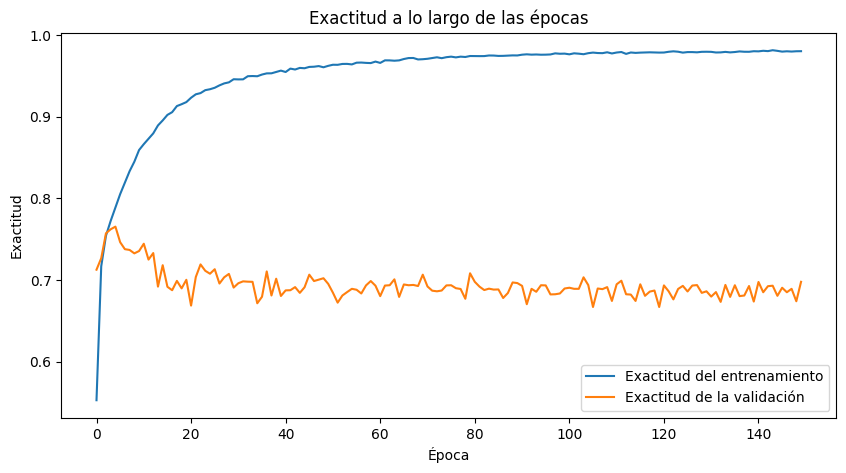
\includegraphics[width=0.65\textwidth]{capitulo5/figuras/exactitud.png}
	\caption{Exacitud a lo largo de las epocas}
	\floatfoot{Fuente: Elaboración propia, generado con matplotlib}
	\label{fig:exactitud}
\end{figure}

\begin{figure}
	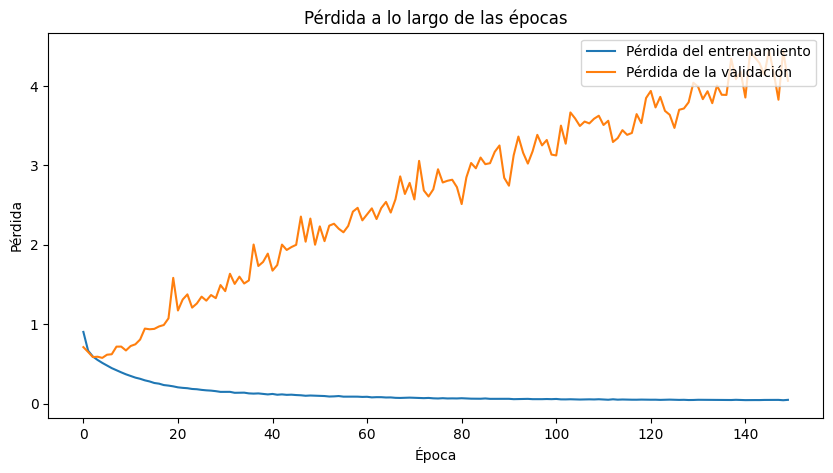
\includegraphics[width=0.65\textwidth]{capitulo5/figuras/perdida.png}
	\caption{Perdida a lo largo de las epocas}
	\floatfoot{Fuente: Elaboración propia, generado con matplotlib}
	\label{fig:perdida}
\end{figure}

\begin{table}[!ht]
	\centering
	\begin{tabular}{|c|c|c|c|c|c|}
		\hline
		\textbf{Nombre del modelo} & \textbf{Precisión} & \textbf{Perdida} & \textbf{Val\_Precisión} & \textbf{Val\_Perdida} & \textbf{Epoca} \\ \hline
		~ & 0.7522 & 0.59 & 0.7650 & 0.5743 & 3 \\ \cline{2-6} 
		cnn\_base\_tt & 0.978 & 0.04 & 0.7128 & 3.3866 & 109 \\ \cline{2-6} 
		~ & 0.9811 & 0.04 & 0.6893 & 3.8825 & 150 \\ \hline
	\end{tabular}
	\caption{Detalle resultados específicos primera iteracion}
	\label{tbl:6}
\end{table}

Modelo base y técnicas de regularización

A continuación, se detallan los modelos base utilizados junto con las técnicas de regularización aplicadas a cada uno. Se eligieron tres tipos de técnicas de regularización: normalización por lotes (batch normalization), regularización L2 y dropout. En esta iteración, se aplicó un tipo de regularización a cada capa convolucional. Los resultados obtenidos se presentan en la tabla \ref{tbl:7} y los detalles  sobre cada modelos a continuación:

\begin{itemize}
\item Modelo cnn\_base\_bn\_tt: Se aplicó normalización por lotes (batch normalization) a cada capa convolucional y a la capa densa intermedia.
\item Modelo cnn\_base\_dp\_tt: Se aplicó un dropout al 30\% a todas las capas convolucionales y un dropout al 50\% a la capa densa intermedia.
\item Modelo cnn\_base\_l2\_tt: Se aplicó regularización L2 con un valor de 0,05 a cada capa convolucional y a la capa densa intermedia.
\end{itemize}

\begin{table}[!ht]
	\centering
	\begin{tabular}{|c|c|c|c|c|c|}
		\hline
		\textbf{Nombre del modelo} & \textbf{Precisión} & \textbf{Perdida} & \textbf{Val\_Precisión} & \textbf{Val\_Perdida} & \textbf{Epoca} \\ \hline
		~ & 0.7890 & 0.52 & 0.7341 & 0.6090 & 4 \\ \cline{2-6} 
		cnn\_base\_bn\_tt & 0.9757 & 0.05 & 0.7272 & 2.8434 & 91 \\ \cline{2-6} 
		~ & 0.9800 & 0.04 & 0.5783 & 3.0617 & 150 \\ \hline
		~ & 0.7752 & 0.56 & 0.7646 & 0.5670 & 7 \\ \cline{2-6} 
		cnn\_base\_dp\_tt & 0.9000 & 0.25 & 0.7400 & 0.9013 & 133 \\ \cline{2-6} 
		~ & 0.9038 & 0.24 & 0.7274 & 0.8862 & 150 \\ \hline
		~ & 0.4185 & 1.02 & 0.4048 & 1.0484 & 123 \\ \cline{2-6} 
		cnn\_base\_l2\_tt & 0.4191 & 1.02 & 0.4048 & 1.0500 & 128 \\ \cline{2-6} 
		~ & 0.4118 & 1.02 & 0.4048 & 1.0503 & 150 \\ \hline
	\end{tabular}
	\caption{Detalle de los modelos base utilizados junto con las técnicas de regularización aplicadas}
	\label{tbl:7}
\end{table}

En los resultados detallados en la tabla \ref{tbl:7}, se observa que los métodos de regularización dropout y batch normalization (BN) retrasaron el sobreajuste. Sin embargo, al considerar el mejor modelo guardado con el menor error, el resultado es casi similar al obtenido por el modelo no regularizado. Por lo tanto, se probó el uso de dos técnicas de regularización simultáneamente en el modelo, manteniendo las mismas características pero modificando la capa densa intermedia a 64 y 32 neuronas en los modelos cnn\_base\_bndp\_64t y cnn\_base\_bndp\_32t, respectivamente. Los detalles y resultados se presentan en la tabla \ref{tbl:8}.

\begin{table}[!ht]
	\centering
	\begin{tabular}{|c|c|c|c|c|c|}
		\hline
		\textbf{Nombre del modelo} & \textbf{Precisión} & \textbf{Perdida} & \textbf{Val\_Precisión} & \textbf{Val\_Perdida} & \textbf{Epoca} \\ \hline
		~ & 0.8135 & 0.47 & 0.7596 & 0.5652 & 22 \\ \cline{2-6}
		cnn\_base\_bndp\_128t & 0.8967 & 0.26 & 0.7463 & 0.7757 & 126 \\ \cline{2-6}
		~ & 0.9029 & 0.25 & 0.7204 & 0.8861 & 150 \\ \hline
		~ & 0.7738 & 0.56 & 0.7777 & 0.5373 & 12 \\ \cline{2-6}
		cnn\_base\_bndp\_64t & 0.8701 & 0.34 & 0.7621 & 0.6211 & 65 \\ \cline{2-6}
		~ & 0.9058 & 0.25 & 0.7531 & 0.7155 & 150 \\ \hline
		~ & 0.8084 & 0.48 & 0.7804 & 0.5584 & 26 \\ \cline{2-6}
		cnn\_base\_bndp\_32t & 0.8580 & 0.37 & 0.7627 & 0.6342 & 56 \\ \cline{2-6}
		~ & 0.8962 & 0.28 & 0.7436 & 0.7562 & 150 \\ \hline
	\end{tabular}
	\caption{Detalle de los modelos base utilizados modificando la capa densa intermedia a 64 y 32 neuronas}
	\label{tbl:8}
\end{table}

Los resultados obtenidos en la tabla algo \ref{tbl:8} demuestran que, sin importar la época, el error en el conjunto de validación no sobrepasará 1.0 y siempre se mantendrá por debajo de ese rango. La precisión en el conjunto de validación se mantendrá siempre por encima de 0.75, siendo la mejor métrica de 0.78, obtenida por el modelo cnn\_base\_bndp\_32t, superando en 2 puntos la precisión del modelo base. Sin embargo, el modelo cnn\_base\_bndp\_64t fue el que obtuvo la menor pérdida.
